\section{寄存器描述}
\regover{
{\hyperref[uart-utx-config]{utx\_config}}&UART TX configuration register
\\
\hline
{\hyperref[uart-urx-config]{urx\_config}}&UART RX configuration register
\\
\hline
{\hyperref[uart-uart-bit-prd]{uart\_bit\_prd}}&UART period control register
\\
\hline
{\hyperref[uart-data-config]{data\_config}}&UART data configuration register
\\
\hline
{\hyperref[uart-utx-ir-position]{utx\_ir\_position}}&UART TX ir position control register
\\
\hline
{\hyperref[uart-urx-ir-position]{urx\_ir\_position}}&UART RX ir position control register
\\
\hline
{\hyperref[uart-urx-rto-timer]{urx\_rto\_timer}}&RTO interrupt control register
\\
\hline
{\hyperref[uart-uart-sw-mode]{uart\_sw\_mode}}&UART SW mode configuration register
\\
\hline
{\hyperref[uart-uart-int-sts]{uart\_int\_sts}}&UART interrupt status
\\
\hline
{\hyperref[uart-uart-int-mask]{uart\_int\_mask}}&UART interrupt mask
\\
\hline
{\hyperref[uart-uart-int-clear]{uart\_int\_clear}}&UART interrupt clear
\\
\hline
{\hyperref[uart-uart-int-en]{uart\_int\_en}}&UART interrupt enable
\\
\hline
{\hyperref[uart-uart-status]{uart\_status}}&UART status control register
\\
\hline
{\hyperref[uart-sts-urx-abr-prd]{sts\_urx\_abr\_prd}}&Auto baud detection control register
\\
\hline
{\hyperref[uart-uart-fifo-config-0]{uart\_fifo\_config\_0}}&UART FIFO configuration register0
\\
\hline
{\hyperref[uart-uart-fifo-config-1]{uart\_fifo\_config\_1}}&UART FIFO configuration register1
\\
\hline
{\hyperref[uart-uart-fifo-wdata]{uart\_fifo\_wdata}}&UART FIFO write data
\\
\hline
{\hyperref[uart-uart-fifo-rdata]{uart\_fifo\_rdata}}&UART FIFO read data
\\
\hline
}

\subsection{utx\_config}
\label{uart-utx-config}
地址:0x4000a000
 \begin{figure}[H]
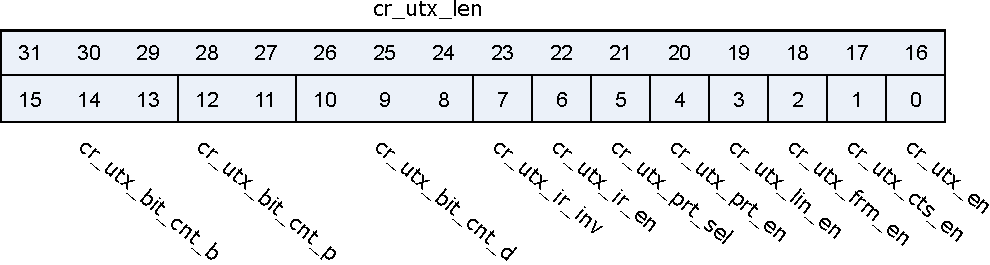
\includegraphics{uart_utx_config.pdf}
\end{figure}

\regdes{31:16&cr\_utx\_len&r/w&16'd0&Length of UART TX data transfer (Unit: character/byte) (Don't-care if cr\_utx\_frm\_en is enabled)\\\hline
15:13&cr\_utx\_bit\_cnt\_b&r/w&3'd4&UART TX BREAK bit count (for LIN protocol) \par Note: Additional 8 bit times will be added since LIN Break field requires at least 13 bit times
\\\hline
12:11&cr\_utx\_bit\_cnt\_p&r/w&2'd1&UART TX STOP bit count (unit: 0.5 bit)\\\hline
10:8&cr\_utx\_bit\_cnt\_d&r/w&3'd7&UART TX DATA bit count for each character\\\hline
7&cr\_utx\_ir\_inv&r/w&1'b0&Inverse signal of UART TX output in IR mode\\\hline
6&cr\_utx\_ir\_en&r/w&1'b0&Enable signal of UART TX IR mode\\\hline
5&cr\_utx\_prt\_sel&r/w&1'b0&Select signal of UART TX parity bit \par 1: Odd parity \par 0: Even parity
\\\hline
4&cr\_utx\_prt\_en&r/w&1'b0&Enable signal of UART TX parity bit\\\hline
3&cr\_utx\_lin\_en&r/w&1'b0&Enable signal of UART TX LIN mode (LIN header will be sent before sending data)\\\hline
2&cr\_utx\_frm\_en&r/w&1'b0&Enable signal of UART TX freerun mode (utx\_end\_int will be disabled)\\\hline
1&cr\_utx\_cts\_en&r/w&1'b0&Enable signal of UART TX CTS flow control function\\\hline
0&cr\_utx\_en&r/w&1'b0&Enable signal of UART TX function \par Asserting this bit will trigger the transaction, and should be de-asserted after finish
\\\hline

}
\subsection{urx\_config}
\label{uart-urx-config}
地址:0x4000a004
 \begin{figure}[H]
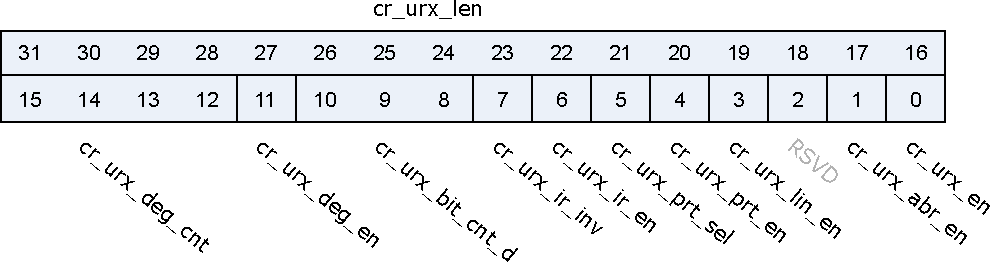
\includegraphics{uart_urx_config.pdf}
\end{figure}

\regdes{31:16&cr\_urx\_len&r/w&16'd0&Length of UART RX data transfer (Unit: character/byte) \par urx\_end\_int will assert when this length is reached
\\\hline
15:12&cr\_urx\_deg\_cnt&r/w&4'd0&De-glitch function cycle count\\\hline
11&cr\_urx\_deg\_en&r/w&1'b0&Enable signal of RXD input de-glitch function\\\hline
10:8&cr\_urx\_bit\_cnt\_d&r/w&3'd7&UART RX DATA bit count for each character\\\hline
7&cr\_urx\_ir\_inv&r/w&1'b0&Inverse signal of UART RX input in IR mode\\\hline
6&cr\_urx\_ir\_en&r/w&1'b0&Enable signal of UART RX IR mode\\\hline
5&cr\_urx\_prt\_sel&r/w&1'b0&Select signal of UART RX parity bit \par 1: Odd parity \par 0: Even parity
\\\hline
4&cr\_urx\_prt\_en&r/w&1'b0&Enable signal of UART RX parity bit\\\hline
3&cr\_urx\_lin\_en&r/w&1'b0&Enable signal of UART RX LIN mode (LIN header will be required and checked before receiving data)\\\hline
2&RSVD& & & \\\hline
1&cr\_urx\_abr\_en&r/w&1'b0&Enable signal of UART RX Auto Baud Rate detection function\\\hline
0&cr\_urx\_en&r/w&1'b0&Enable signal of UART RX function\\\hline

}
\subsection{uart\_bit\_prd}
\label{uart-uart-bit-prd}
地址:0x4000a008
 \begin{figure}[H]
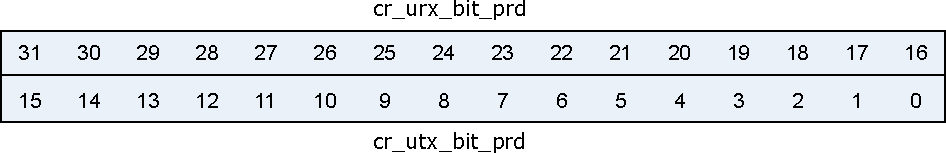
\includegraphics{uart_uart_bit_prd.pdf}
\end{figure}

\regdes{31:16&cr\_urx\_bit\_prd&r/w&16'd255&Period of each UART RX bit, related to baud rate\\\hline
15:0&cr\_utx\_bit\_prd&r/w&16'd255&Period of each UART TX bit, related to baud rate\\\hline

}
\subsection{data\_config}
\label{uart-data-config}
地址:0x4000a00c
 \begin{figure}[H]
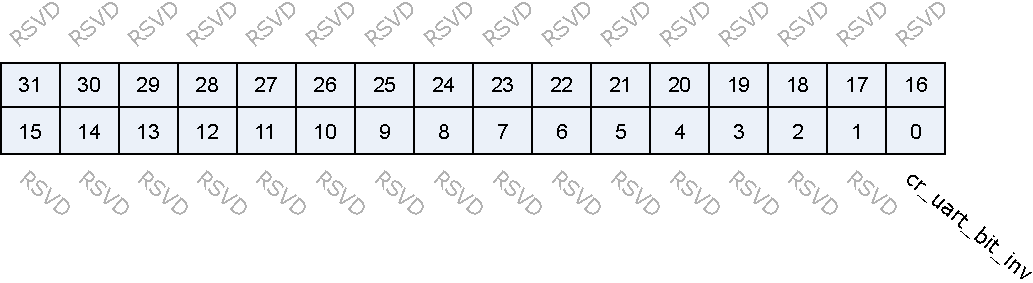
\includegraphics{uart_data_config.pdf}
\end{figure}

\regdes{31:1&RSVD& & & \\\hline
0&cr\_uart\_bit\_inv&r/w&1'b0&Bit-inverse signal for each data byte \par 0: Each byte is sent out LSB-first \par 1: Each byte is sent out MSB-first
\\\hline

}
\subsection{utx\_ir\_position}
\label{uart-utx-ir-position}
地址:0x4000a010
 \begin{figure}[H]
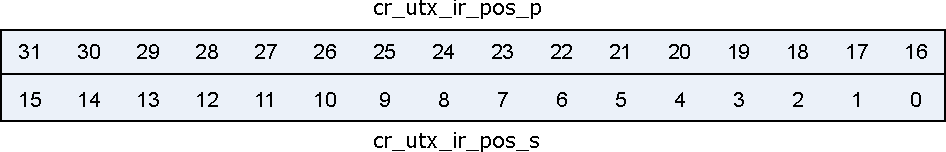
\includegraphics{uart_utx_ir_position.pdf}
\end{figure}

\regdes{31:16&cr\_utx\_ir\_pos\_p&r/w&16'd159&STOP position of UART TX IR pulse\\\hline
15:0&cr\_utx\_ir\_pos\_s&r/w&16'd112&START position of UART TX IR pulse\\\hline

}
\subsection{urx\_ir\_position}
\label{uart-urx-ir-position}
地址:0x4000a014
 \begin{figure}[H]
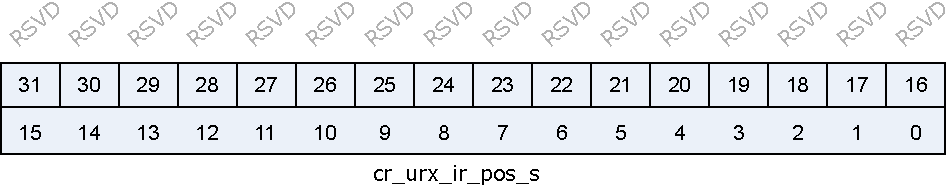
\includegraphics{uart_urx_ir_position.pdf}
\end{figure}

\regdes{31:16&RSVD& & & \\\hline
15:0&cr\_urx\_ir\_pos\_s&r/w&16'd111&START position of UART RXD pulse recovered from IR signal\\\hline

}
\subsection{urx\_rto\_timer}
\label{uart-urx-rto-timer}
地址:0x4000a018
 \begin{figure}[H]
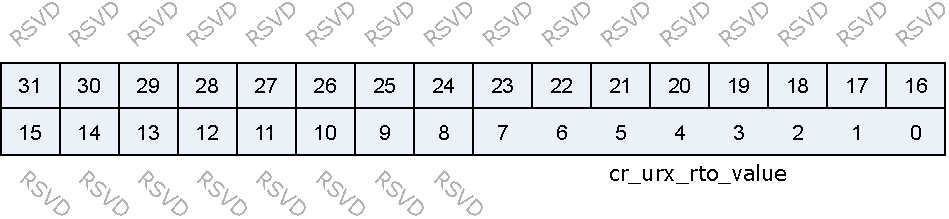
\includegraphics{uart_urx_rto_timer.pdf}
\end{figure}

\regdes{31:8&RSVD& & & \\\hline
7:0&cr\_urx\_rto\_value&r/w&8'd15&Time-out value for triggering RTO interrupt (unit: bit time)\\\hline

}
\subsection{uart\_sw\_mode}
\label{uart-uart-sw-mode}
地址:0x4000a01c
 \begin{figure}[H]
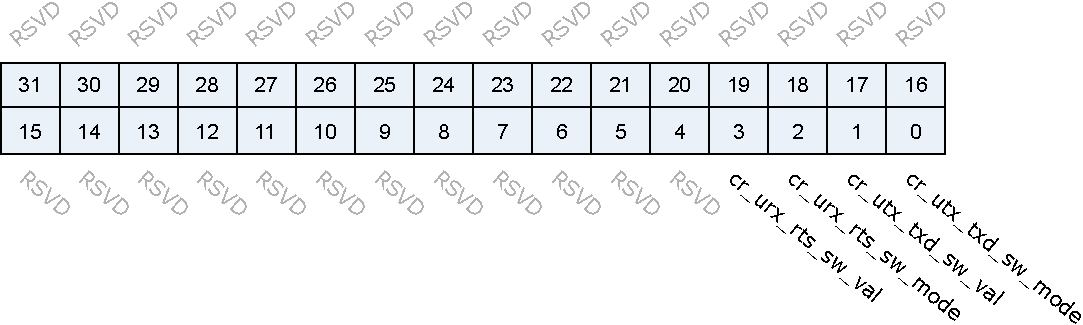
\includegraphics{uart_uart_sw_mode.pdf}
\end{figure}

\regdes{31:4&RSVD& & & \\\hline
3&cr\_urx\_rts\_sw\_val&r/w&1'b0&UART RX RTS output SW control value\\\hline
2&cr\_urx\_rts\_sw\_mode&r/w&1'b0&UART RX RTS output SW control mode\\\hline
1&cr\_utx\_txd\_sw\_val&r/w&1'b0&UART TX TXD output SW control value\\\hline
0&cr\_utx\_txd\_sw\_mode&r/w&1'b0&UART TX TXD output SW control mode\\\hline

}
\subsection{uart\_int\_sts}
\label{uart-uart-int-sts}
地址:0x4000a020
 \begin{figure}[H]
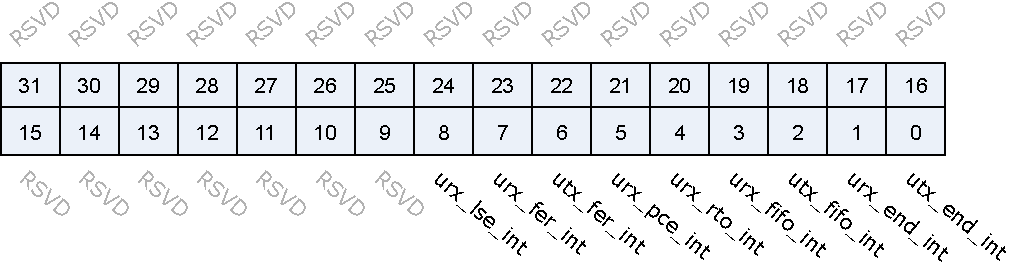
\includegraphics{uart_uart_int_sts.pdf}
\end{figure}

\regdes{31:9&RSVD& & & \\\hline
8&urx\_lse\_int&r&1'b0&UART RX LIN mode sync field error interrupt\\\hline
7&urx\_fer\_int&r&1'b0&UART RX FIFO error interrupt, auto-cleared when FIFO overflow/underflow error flag is cleared\\\hline
6&utx\_fer\_int&r&1'b0&UART TX FIFO error interrupt, auto-cleared when FIFO overflow/underflow error flag is cleared\\\hline
5&urx\_pce\_int&r&1'b0&UART RX parity check error interrupt\\\hline
4&urx\_rto\_int&r&1'b0&UART RX Time-out interrupt\\\hline
3&urx\_fifo\_int&r&1'b0&UART RX FIFO ready (rx\_fifo\_cnt > rx\_fifo\_th) interrupt, auto-cleared when data is popped\\\hline
2&utx\_fifo\_int&r&1'b0&UART TX FIFO ready (tx\_fifo\_cnt > tx\_fifo\_th) interrupt, auto-cleared when data is pushed\\\hline
1&urx\_end\_int&r&1'b0&UART RX transfer end interrupt (set according to cr\_urx\_len)\\\hline
0&utx\_end\_int&r&1'b0&UART TX transfer end interrupt (set according to cr\_utx\_len)\\\hline

}
\subsection{uart\_int\_mask}
\label{uart-uart-int-mask}
地址:0x4000a024
 \begin{figure}[H]
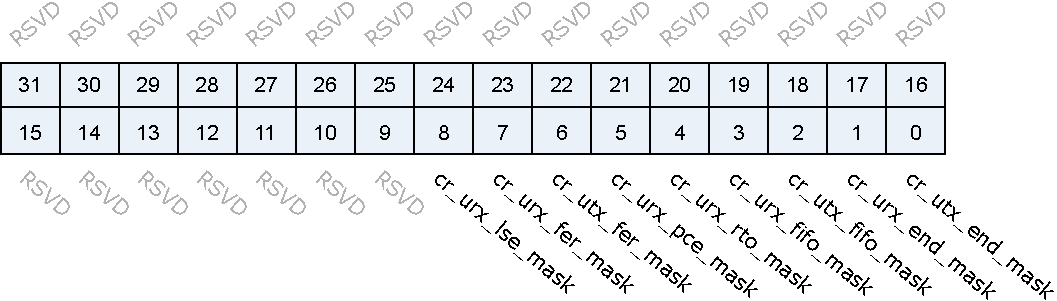
\includegraphics{uart_uart_int_mask.pdf}
\end{figure}

\regdes{31:9&RSVD& & & \\\hline
8&cr\_urx\_lse\_mask&r/w&1'b1&Interrupt mask of urx\_lse\_int\\\hline
7&cr\_urx\_fer\_mask&r/w&1'b1&Interrupt mask of urx\_fer\_int\\\hline
6&cr\_utx\_fer\_mask&r/w&1'b1&Interrupt mask of utx\_fer\_int\\\hline
5&cr\_urx\_pce\_mask&r/w&1'b1&Interrupt mask of urx\_pce\_int\\\hline
4&cr\_urx\_rto\_mask&r/w&1'b1&Interrupt mask of urx\_rto\_int\\\hline
3&cr\_urx\_fifo\_mask&r/w&1'b1&Interrupt mask of urx\_fifo\_int\\\hline
2&cr\_utx\_fifo\_mask&r/w&1'b1&Interrupt mask of utx\_fifo\_int\\\hline
1&cr\_urx\_end\_mask&r/w&1'b1&Interrupt mask of urx\_end\_int\\\hline
0&cr\_utx\_end\_mask&r/w&1'b1&Interrupt mask of utx\_end\_int\\\hline

}
\subsection{uart\_int\_clear}
\label{uart-uart-int-clear}
地址:0x4000a028
 \begin{figure}[H]
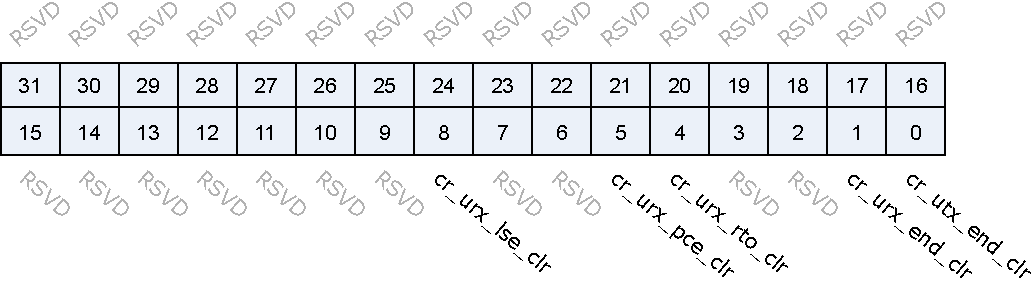
\includegraphics{uart_uart_int_clear.pdf}
\end{figure}

\regdes{31:9&RSVD& & & \\\hline
8&cr\_urx\_lse\_clr&w1c&1'b0&Interrupt clear of urx\_lse\_int\\\hline
7:6&RSVD& & & \\\hline
5&cr\_urx\_pce\_clr&w1c&1'b0&Interrupt clear of urx\_pce\_int\\\hline
4&cr\_urx\_rto\_clr&w1c&1'b0&Interrupt clear of urx\_rto\_int\\\hline
3:2&RSVD& & & \\\hline
1&cr\_urx\_end\_clr&w1c&1'b0&Interrupt clear of urx\_end\_int\\\hline
0&cr\_utx\_end\_clr&w1c&1'b0&Interrupt clear of utx\_end\_int\\\hline

}
\subsection{uart\_int\_en}
\label{uart-uart-int-en}
地址:0x4000a02c
 \begin{figure}[H]
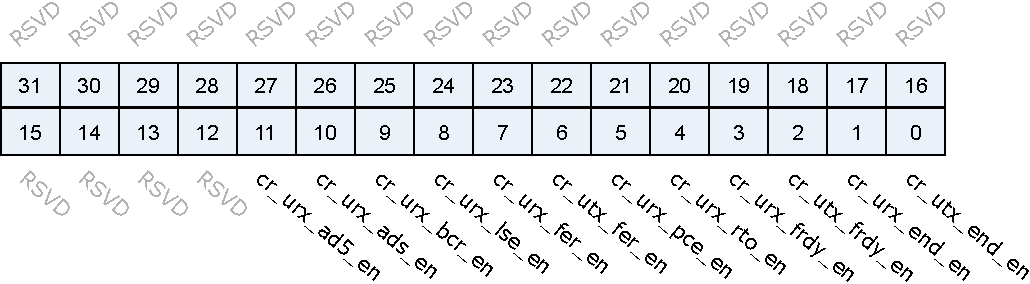
\includegraphics{uart_uart_int_en.pdf}
\end{figure}

\regdes{31:9&RSVD& & & \\\hline
8&cr\_urx\_lse\_en&r/w&1'b1&Interrupt enable of urx\_lse\_int\\\hline
7&cr\_urx\_fer\_en&r/w&1'b1&Interrupt enable of urx\_fer\_int\\\hline
6&cr\_utx\_fer\_en&r/w&1'b1&Interrupt enable of utx\_fer\_int\\\hline
5&cr\_urx\_pce\_en&r/w&1'b1&Interrupt enable of urx\_pce\_int\\\hline
4&cr\_urx\_rto\_en&r/w&1'b1&Interrupt enable of urx\_rto\_int\\\hline
3&cr\_urx\_fifo\_en&r/w&1'b1&Interrupt enable of urx\_fifo\_int\\\hline
2&cr\_utx\_fifo\_en&r/w&1'b1&Interrupt enable of utx\_fifo\_int\\\hline
1&cr\_urx\_end\_en&r/w&1'b1&Interrupt enable of urx\_end\_int\\\hline
0&cr\_utx\_end\_en&r/w&1'b1&Interrupt enable of utx\_end\_int\\\hline

}
\subsection{uart\_status}
\label{uart-uart-status}
地址:0x4000a030
 \begin{figure}[H]
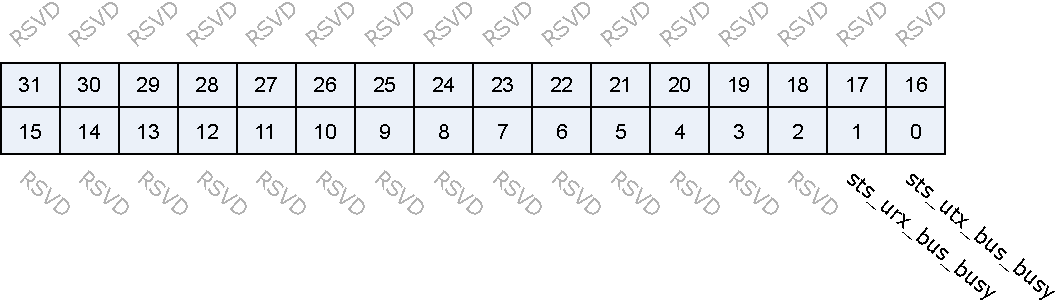
\includegraphics{uart_uart_status.pdf}
\end{figure}

\regdes{31:2&RSVD& & & \\\hline
1&sts\_urx\_bus\_busy&r&1'b0&Indicator of UART RX bus busy\\\hline
0&sts\_utx\_bus\_busy&r&1'b0&Indicator of UART TX bus busy\\\hline

}
\subsection{sts\_urx\_abr\_prd}
\label{uart-sts-urx-abr-prd}
地址:0x4000a034
 \begin{figure}[H]
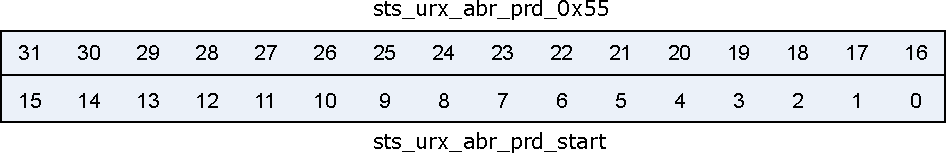
\includegraphics{uart_sts_urx_abr_prd.pdf}
\end{figure}

\regdes{31:16&sts\_urx\_abr\_prd\_0x55&r&16'd0&Bit period of Auto Baud Rate detection using codeword 0x55\\\hline
15:0&sts\_urx\_abr\_prd\_start&r&16'd0&Bit period of Auto Baud Rate detection using START bit\\\hline

}
\subsection{uart\_fifo\_config\_0}
\label{uart-uart-fifo-config-0}
地址:0x4000a080
 \begin{figure}[H]
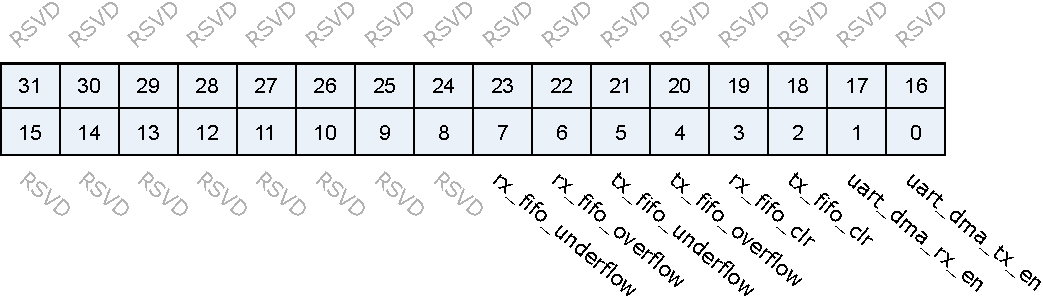
\includegraphics{uart_uart_fifo_config_0.pdf}
\end{figure}

\regdes{31:8&RSVD& & & \\\hline
7&rx\_fifo\_underflow&r&1'b0&Underflow flag of RX FIFO, can be cleared by rx\_fifo\_clr\\\hline
6&rx\_fifo\_overflow&r&1'b0&Overflow flag of RX FIFO, can be cleared by rx\_fifo\_clr\\\hline
5&tx\_fifo\_underflow&r&1'b0&Underflow flag of TX FIFO, can be cleared by tx\_fifo\_clr\\\hline
4&tx\_fifo\_overflow&r&1'b0&Overflow flag of TX FIFO, can be cleared by tx\_fifo\_clr\\\hline
3&rx\_fifo\_clr&w1c&1'b0&Clear signal of RX FIFO\\\hline
2&tx\_fifo\_clr&w1c&1'b0&Clear signal of TX FIFO\\\hline
1&uart\_dma\_rx\_en&r/w&1'b0&Enable signal of dma\_rx\_req/ack interface\\\hline
0&uart\_dma\_tx\_en&r/w&1'b0&Enable signal of dma\_tx\_req/ack interface\\\hline

}
\subsection{uart\_fifo\_config\_1}
\label{uart-uart-fifo-config-1}
地址:0x4000a084
 \begin{figure}[H]
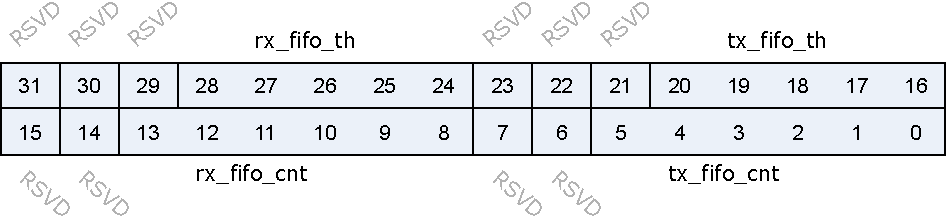
\includegraphics{uart_uart_fifo_config_1.pdf}
\end{figure}

\regdes{31&RSVD& & & \\\hline
30:24&rx\_fifo\_th&r/w&7'd0&RX FIFO threshold, dma\_rx\_req will not be asserted if tx\_fifo\_cnt is less than this value\\\hline
23&RSVD& & & \\\hline
22:16&tx\_fifo\_th&r/w&7'd0&TX FIFO threshold, dma\_tx\_req will not be asserted if tx\_fifo\_cnt is less than this value\\\hline
15:8&rx\_fifo\_cnt&r&8'd0&RX FIFO available count\\\hline
7:0&tx\_fifo\_cnt&r&8'd128&TX FIFO available count\\\hline

}
\subsection{uart\_fifo\_wdata}
\label{uart-uart-fifo-wdata}
地址:0x4000a088
 \begin{figure}[H]
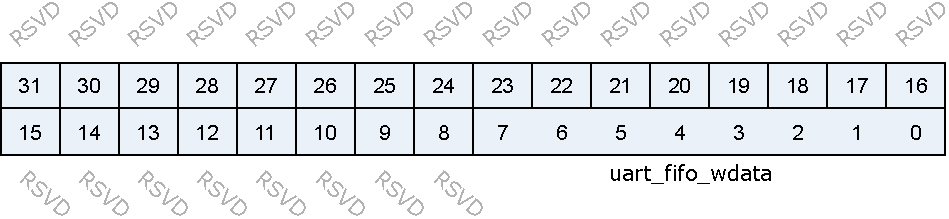
\includegraphics{uart_uart_fifo_wdata.pdf}
\end{figure}

\regdes{31:8&RSVD& & & \\\hline
7:0&uart\_fifo\_wdata&w&x&\\\hline

}
\subsection{uart\_fifo\_rdata}
\label{uart-uart-fifo-rdata}
地址:0x4000a08c
 \begin{figure}[H]
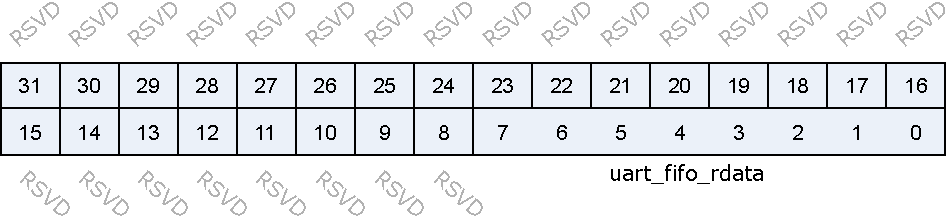
\includegraphics{uart_uart_fifo_rdata.pdf}
\end{figure}

\regdes{31:8&RSVD& & & \\\hline
7:0&uart\_fifo\_rdata&r&8'h0&\\\hline

}
